%\documentclass[conference]{IEEEtran}
\documentclass[10pt,conference,anonymous]{IEEEtran}
\IEEEoverridecommandlockouts

%% Marcelo added this
\makeatletter
\renewcommand\footnoterule{%
  \kern-3\p@
  \hrule\@width.4\columnwidth
  \kern2.6\p@}
  \makeatother




\usepackage{inconsolata}
\usepackage{listings}

\lstset{language=Java,
basicstyle=\ttfamily\scriptsize,
%basicstyle=\ttfamily,
keywordstyle=\color{javapurple}\bfseries,
stringstyle=\color{pblue},
commentstyle=\color{javagreen},
morecomment=[s][\color{javadocblue}]{/**}{*/},
morecomment=[s][\color{gray}]{@}{\ },
numbers=left,
numberstyle=\tiny\color{black},
stepnumber=2,
numbersep=8pt,
tabsize=4,
showspaces=false,
showstringspaces=false,
breaklines=true,}

%%%%%%%%%%%%%%%%%%%%%%%%%%%%%%%%%%




\usepackage{adjustbox} % ajustar tabela ao tamanho da pagina

\usepackage{tikz}
\usetikzlibrary{matrix,fit,shapes,calc,positioning,shadows,arrows,shapes,backgrounds,decorations.markings,fadings}
\usepackage{graphicx}
\usepackage{multirow}
\usepackage[caption=false, font=footnotesize]{subfig}
\usepackage{wrapfig}
\usepackage{enumitem}
\usepackage{url}
%% helpers
\newcommand{\js}{JS}
\newcommand{\javascript}{JavaScript}
\newcommand{\es}{ES}
\newcommand{\ecmascript}{\es{}}
\newcommand{\tname}{TNAME}
\newcommand{\Comment}[1]{}
\newcommand{\numsubjects}{5}
\newcommand{\etal}{and colleagues'}
\newcommand{\ie}{i.e.}
\newcommand{\eg}{e.g.}
\newcommand{\cmark}{\ding{51}}%
\newcommand{\xmark}{{\color{red}\ding{55}}}%
\newcommand{\pGoodGood}{$\mathit{P}${\small\cmark\!\cmark}}%
\newcommand{\pGoodBad}{$\mathit{P}${\small\cmark\!\xmark}}%
\newcommand{\pBadDontCare}{$\mathit{P_?}$}%
\newcommand{\sfl}{SFL\xspace}
\newcommand{\ddg}{DDG\xspace}
\newcommand{\totfiles}{$\sim$38K}

%% annotations
\newif\ifdraftmode
%% Comment or uncomment the \draftmodetrue line.
\draftmodetrue
\ifdraftmode
 \newcommand{\Fix}[1]{\textbf{[[}{\color{red} #1}\textbf{]]}}
 \newcommand{\Mar}[1]{\textbf{[[Marcelo: }{\color{magenta} #1}\textbf{]]}}
 \newcommand{\Igor}[1]{\textbf{[[Igor: }{\color{blue} #1}\textbf{]]}}
 \newcommand{\note}[1]{\todo[inline,color=red!30,caption={}]{#1}}
\else
 \newcommand{\Fix}[1]{\relax}
 \newcommand{\Mar}[1]{\relax}
 \newcommand{\Igor}[1]{\relax}
 \newcommand{\note}[1]{\relax}
\fi

% For submitted version only.
\pagenumbering{arabic}

% Uncomment this if you need more space
%% \makeatletter
%% \def\@copyrightspace{\enlargethispage{-10pt}\relax}
%% \makeatother

\newcommand{\codesize}{\small}
\newcommand{\CodeIn}[1]{\mcodeid{#1}}
\newcommand{\CodeInM}[1]{\mcodeid{#1}}
% \|name| or \mathid{name} denotes identifiers and slots in formulas
\def\|#1|{\mathid{#1}}
\newcommand{\mathid}[1]{\ensuremath{\mathit{#1}}}
% \<name> or \codeid{name} denotes computer code identifiers
\def\<#1>{\codeid{#1}}
\newcommand{\codeid}[1]{\ifmmode{\mbox{\codesize\ttfamily{#1}}}\else{\codesize\ttfamily #1}\fi}
\def\<#1>{\mcodeid{#1}}
\newcommand{\mcodeid}[1]{\mbox{\codesize\ttfamily{#1}}}

%% thumbs up down
\newcommand*{\RightThumbsUpAux}[1]{%
  \begingroup
    \sbox0{Ag}%
    \raisebox{-\dp0}{%
      \includegraphics[{%
        height=\dimexpr\dp0+\ht0\relax,
        #1%
      }]{thumbsup.pdf}%
    }%
  \endgroup
}
\newcommand*{\RightThumbsUp}{%
  \RightThumbsUpAux{}%
}
\newcommand*{\RightThumbsDown}{%
  \RightThumbsUpAux{origin=c,angle=180}%
}
\newcommand*{\LeftThumbsUp}{%
  \scalebox{-1}[1]{\RightThumbsUp}%
}
\newcommand*{\LeftThumbsDown}{%
  \scalebox{-1}[1]{\RightThumbsDown}%
}

\newcommand{\checkm}{Y}
\newcommand{\crossmark}{N}
%\begin{wraptable}[20]{t}[0pt]{0.5\textwidth}

\newcommand{\totalTestFiles}{38,369}
\newcommand{\totalTestFilesCompileInAll}{35,939}
\newcommand{\totalTestFilesPassInAll}{24,493}
\newcommand{\nofuzzAll}{209}
\newcommand{\nofuzzBugs}{\Fix{XX}}
\newcommand{\nofuzzDuplicates}{63}
\newcommand{\nofuzzFalsePositives}{24}
\newcommand{\nofuzzHITotal}{177}
\newcommand{\nofuzzLOTotal}{32}
\newcommand{\nofuzzTotalFiles}{977} % conflicting files
\newcommand{\nofuzzFilesHI}{940} % conflicting files HI
\newcommand{\nofuzzFilesLO}{37} % conflicting files LO

\newcommand{\nofuzzBucketsBugsHI}{\Fix{124}} % buckets reported (including dups)
\newcommand{\nofuzzBucketsBugsLO}{\Fix{11}} % buckets reported
\newcommand{\nofuzzDupsHI}{\Fix{X}}
\newcommand{\nofuzzDupsLO}{\Fix{Y}}

% continue updating bugs table
\newcommand{\tableBugsNum}{\Fix{26}}

%% anonymize

\newcommand{\anonym}[1]{{\tiny\colorbox{black}{#1}}}

%% names
\newcommand{\radamsa}{radamsa}
\newcommand{\quickfuzz}{quickfuzz}

\newcommand{\jsc}{JavaScriptCore}
\newcommand{\veight}{V8}
\newcommand{\chakra}{Chakra}
\newcommand{\smonkey}{SpiderMonkey}
\newcommand{\jerry}{JerryScript}

\newcommand{\lo}{lo}
\newcommand{\hi}{hi}


\begin{document}

\title{Finding Functional Bugs in JavaScript Engines with Differential
  Testing---an Experience Report}

%% \author{
%% \IEEEauthorblockN{Sabrina Souto}
%% \IEEEauthorblockA{State University of Para\'iba\\
%% Para\'iba, Brazil\\
%% sabrinadfs@gmail.com}
%% \and
%% \IEEEauthorblockN{Marcelo d'Amorim}
%% \IEEEauthorblockA{Federal University of Pernambuco\\
%%   Pernambuco, Brazil\\
%%   damorim@cin.ufpe.br}
%% \and
%% \IEEEauthorblockN{Rohit Gheyi}
%% \IEEEauthorblockA{Federal University of Campina Grande\\
%%   Para\'iba, Brazil\\
%%   rohit@dsc.ufcg.edu.br}
%% }

\maketitle

\begin{abstract}
\end{abstract}

\begin{IEEEkeywords}
...
\end{IEEEkeywords}

\section{Introduction}

JavaScript (\js{}) is one of the most popular programming languages of
today~\cite{business-insider,stackify}. The \js{} specification
changes relatively frequently to accommodate the pressing demands of
the community. For example, the JS specification went through a severe
change recently called by the name of ECMAScript6
(ES6)~\cite{es6-features}.  These changes often entail sensible
changes in engine implementations~\cite{kangax} that could lead to
errors, including regressions. Automated techniques can help finding
bugs, but the lack of executable specifications limits their ability
to detect errors not manifested by universal oracles.

This paper reports on a study to find those kinds of bugs in
JavaScript engines. The goal of the study is to improve quality of
existing \js{} engines by improving the bug-finding process. We used
differential testing~\cite{Brumley-etal-ss07}, a technique that has
been applied in a variety of
contexts~\cite{Yang-etal-pldi11,Chen-etal-fse2015,Argyros-etla-ccs16,Chen-etal-pldi16,petsios-etal-sp2017,SivakornAPKJ17}
to address the oracle problem. Differential testing leverages the
diversity across system's implementations to detect anomalous
behavior. \Mar{this needs work$\rightarrow$}
\Fix{but it has not been thoroughly explored to find functional bugs in JS
engines. The closest work was done by Patra and
Pradel~\cite{patra2016learning}, where they evaluated their proposed
language-agnostic fuzzer to find cross-browser HTML+JS
discrepancies. This project aims at building and evaluating an
infrastructure for differential testing of runtime engines, such as
the JS engine or WebAssembly's. The sensible parts of the
infrastructure are the checks of input validity (as to reduce
waste/cost) and output correctness (as to reduce false positives).}

\section{Infrastructure}
\label{sec:design}


%\begin{wrapfigure}[10]{r}[0pt]{0.45\textwidth}
\begin{figure}[t]
  \centering
%  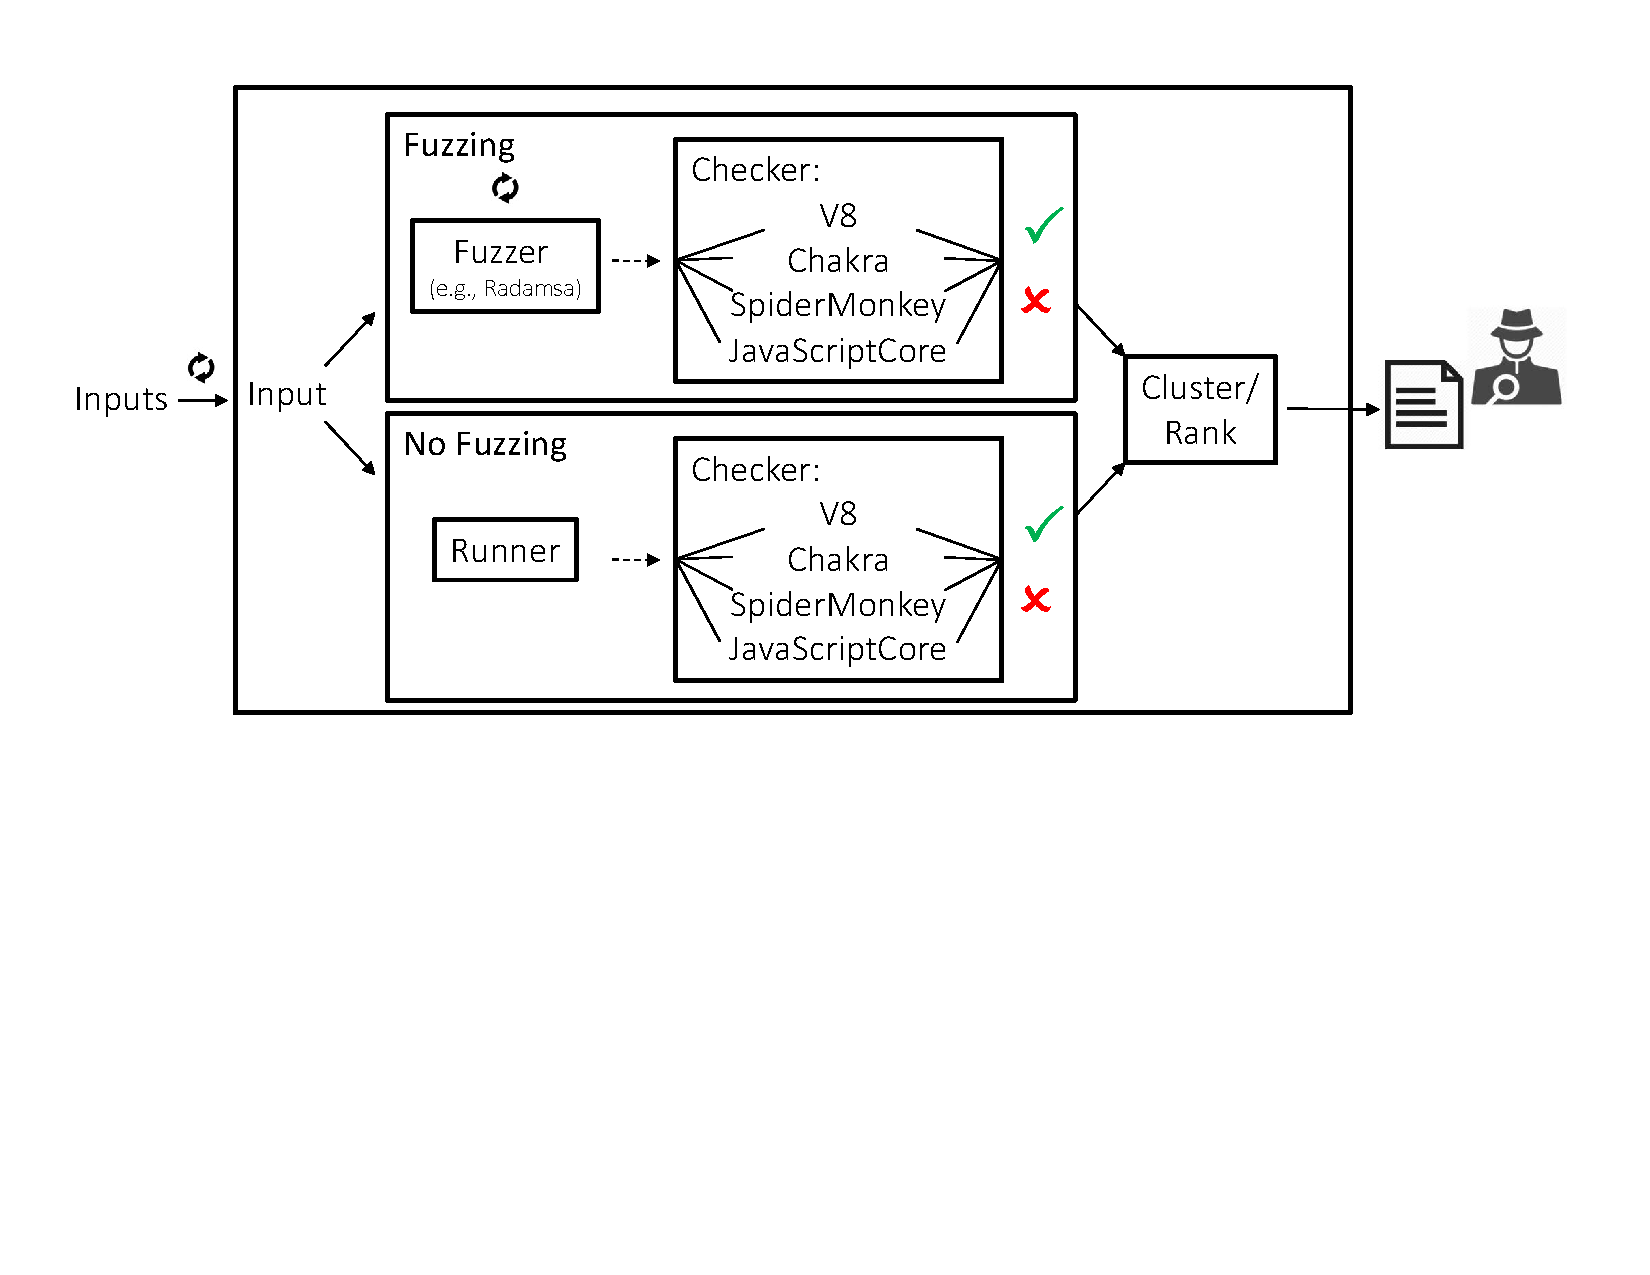
\includegraphics[trim=20 350 200
%    0,clip,width=0.35\textwidth]{google-awards-workflow}
  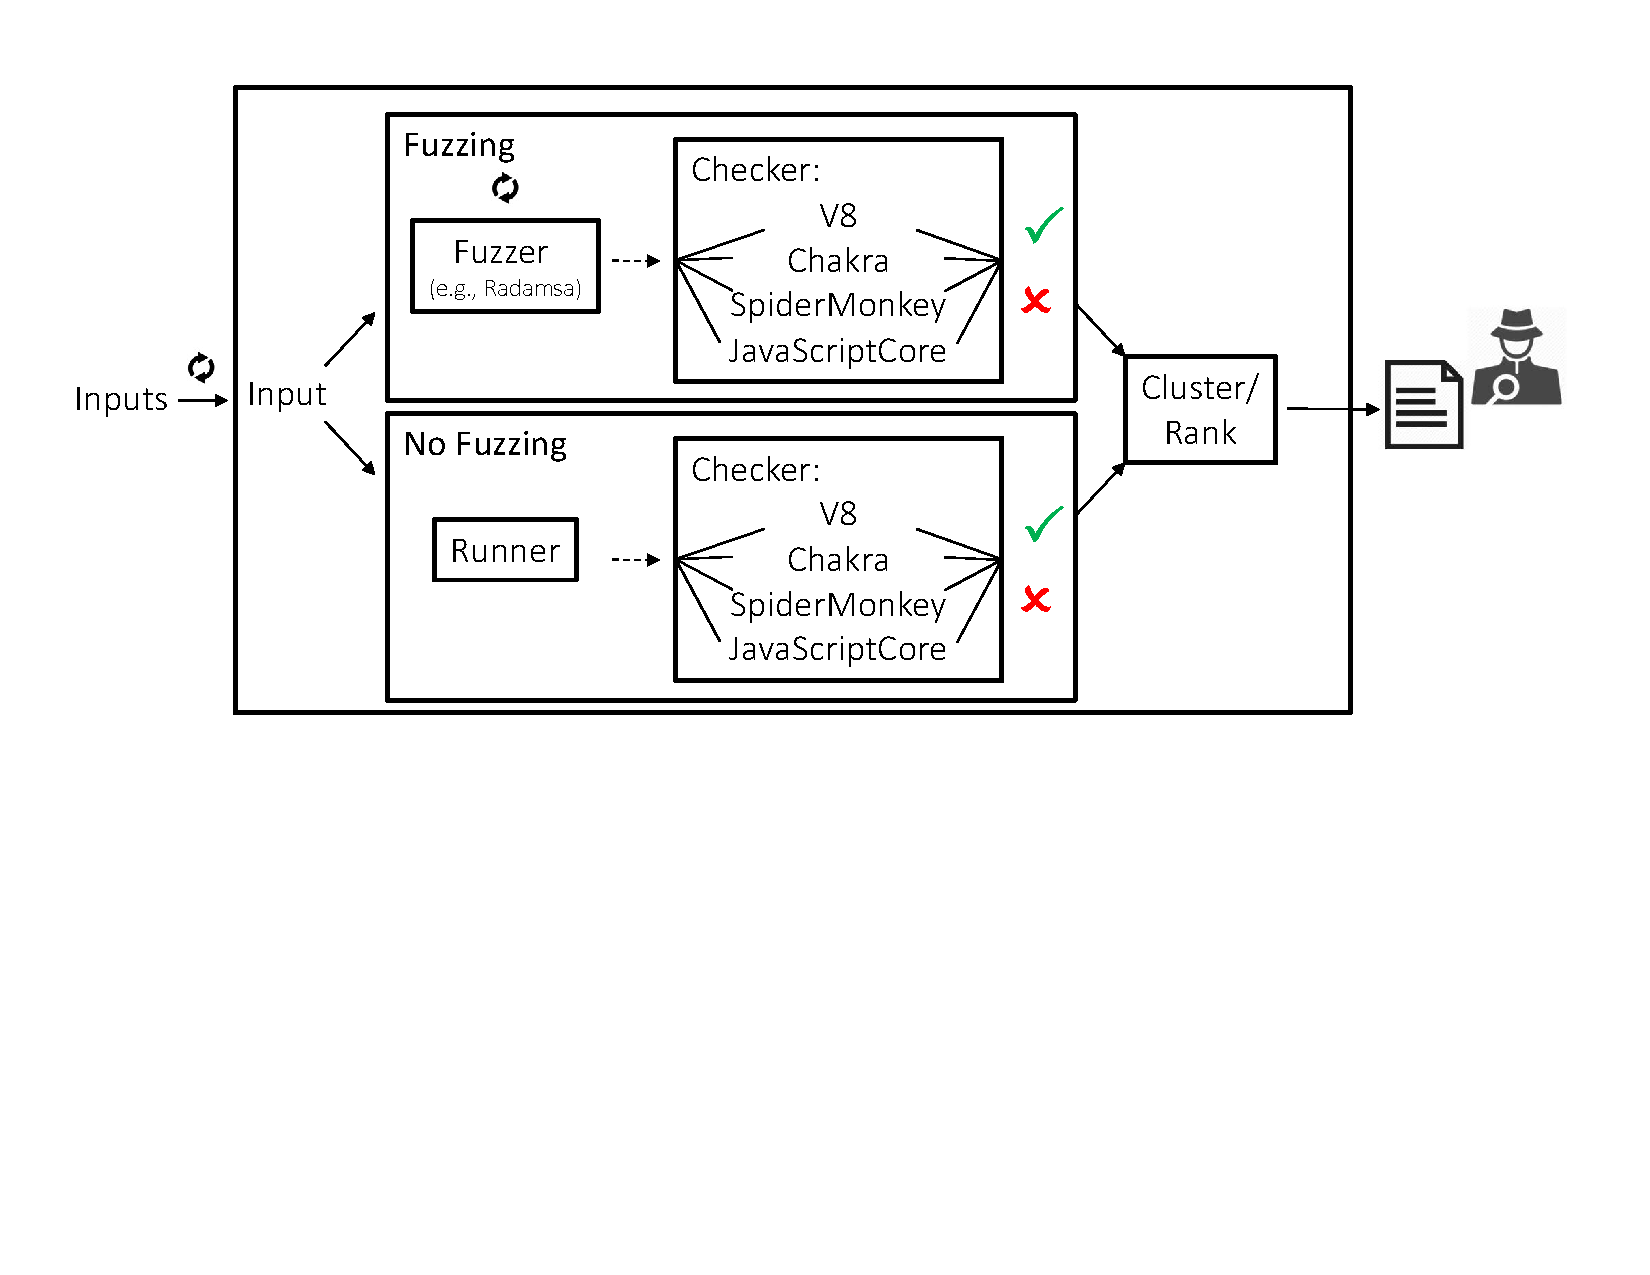
\includegraphics[trim=0 250 0 0,clip,width=0.5\textwidth]{google-awards-workflow}  
  \caption{\label{fig:workflow}Infrastructure.}
\end{figure}

Figure~\ref{fig:workflow} illustrates the workflow of the
infrastructure we used in this study. Boxes denote encapsulation,
arrowed lines indicate control flow (dashed) and data flow (filled),
and the cyclic icons denote repetition. In this case, it indicates
that each test file will be proceseed in separate and, if fuzzing is
selected, a single file can be processed multiple times--one for each
of its fuzzed variants. The bug-finding process takes on input JS
files from regression test suites of various JS
engines. Table~\ref{tab:test-suites} shows the JS sources we mined
from online repositories of various open-source engines. Overall, we
found a total of \Fix{XX} JS files.

\begin{table}[h]
  \centering
  \caption{\label{tab:test-suites}Test Suites\Fix{use path in the repo}}
  \begin{tabular}{ccc}
    \toprule
    TestSuite & Source & \# JS files \\
    \midrule
    \Fix{duktape} & - & - \\
    \Fix{jerryjs} & - & - \\
    \Fix{jsi} & - & - \\
    \Fix{tiny} & - & - \\
    \Fix{mozilla} & - & - \\
    v8.test.benchmarks.data & - & - \\
    webkit.jstests.es6 & - & - \\
    webkit.jstests.microbenchmarks & - & - \\
   \bottomrule     
  \end{tabular}
\end{table}


The bug-finding process works as follows.  Considering the case
fuzzing is not selected, as illustrated in the inner box at the bottom
of the figure, the oracle checks whether or not the output
produced for that file is consistent across all engine
implementations. In case the test passes in all engines or fails in
all engines (\ie{}, the output is consistent), the infrastructure
discards the corresponding input. Otherwise, it considers the input as
potentially fault-revealing; hence interesting for human
inspection. Considering the case where fuzzing~\cite{fuzz-testing-history}
is selected, new inputs are obtained from a given input using some
off-the-shelf fuzzer\footnote{Several fuzzing methods have been proposed in
the past, varying with respect to how new inputs are generated (\eg{},
coverage-based~\cite{afl,honggfuzz},
grammar-based~\cite{grammarinator,jsfunfuzz}, and
random-based~\cite{radamsa}).}. The workflow is similar to that of no
fuzzing. In this case, however, multiple warnings can be produced for
a given seed input.

The infrastructure outputs a list of warnings for human inspection.
To reduce the number of false alarms, we clustered warnings in two
groups, reflecting their likelihood to manifest a real bug. The HI
group includes those inputs where execution manifests anomaly in the
test code (or its close neighborhood) as opposed to some internal JS
function. The rationale is that the test in this group executed
without violating any internal checks of the API.
The LO group, in contrast, includes those cases where the anomaly
was observed executing some JS function. We found that engine
implementations often check pre-conditions of API functions
differently, leading to premature failures which manifest themselves as
discrepancy in our infrastructure. Although we did find real bugs from
warnings in the LO group, the proportion was much lower compared to the HI
group--only 12\% of the reals bugs we found originated from the LO
category. \Mar{show real examples of HI and LO and provide the
  rationale for such classification.} \Mar{can we detect dups mining
  issue trackers?}

\begin{table*}[ht!]
  \vspace{-3ex}
%  \scriptsize
  \centering
  \caption{List of bug reports issued by our team from April 12 to May
    24, 2018.}
  \label{tab:bugs}
  \begin{tabular}{cccccc}
    \toprule
    Issue\#    & Date & Fuzz & Engine  & Status  & \multicolumn{1}{c}{Url}  \\
    \midrule    
    1  & 4/12 & \checkm & Chakra   & \textbf{Fixed}  & \href{https://github.com/Microsoft/ChakraCore/issues/4978}{\#4978}      \\ 
    2  & 4/12 & \checkm & Chakra   & Rejected  & \href{https://github.com/Microsoft/ChakraCore/issues/4979}{\#4979}      \\
    3  & 4/14 & \checkm & JavascriptCore  & New & \href{https://bugs.webkit.org/show\_bug.cgi?id=184629}{\#184629}        \\
    4  & 4/18 & \crossmark & JavascriptCore  & New  & \href{https://bugs.webkit.org/show\_bug.cgi?id=184749}{\#184749}        \\
    5  & 4/23 & \crossmark & Chakra  & \textbf{Confirmed}  & \href{https://github.com/Microsoft/ChakraCore/issues/5033}{\#5033}       \\
    6  & 4/25 & \checkm & Chakra  & \textbf{Fixed}     & \href{https://github.com/Microsoft/ChakraCore/issues/5038}{\#5038}      \\
    7  & 4/29 & \crossmark & Chakra  & \textbf{Confirmed}   &
    \href{https://github.com/Microsoft/ChakraCore/issues/5065}{\#5065}
    \\
    \midrule
    \multirow{2}{*}{8}  & \multirow{2}{*}{4/29} &  \multirow{2}{*}{\crossmark} & Chakra & \textbf{Confirmed} &    \href{https://github.com/Microsoft/ChakraCore/issues/5067}{\#5067} \\
                        &  &                       &
    JavascriptCore & New &    \href{https://bugs.webkit.org/show\_bug.cgi?id=185130}{\#185130}    \\
    \midrule    
    9  & 4/29 & \checkm & JavascriptCore  & New  &    \href{https://bugs.webkit.org/show\_bug.cgi?id=185127}{\#185127}    \\
    \midrule    
    \multirow{2}{*}{10} & \multirow{2}{*}{4/30}  & \multirow{2}{*}{\checkm} & Chakra & \textbf{Confirmed} &    \href{https://github.com/Microsoft/ChakraCore/issues/5076}{\#5076} \\    
                        &                        &        &
    JavascriptCore & New &
    \href{https://bugs.webkit.org/show\_bug.cgi?id=185156}{\#185156}
    \\
    \midrule    
    11 & 5/02 & \checkm & JavascriptCore  & New & \href{https://bugs.webkit.org/show\_bug.cgi?id=185197}{\#185197}\\
    12 & 5/02 & \crossmark & JavascriptCore & New  & \href{https://bugs.webkit.org/show\_bug.cgi?id=185208}{\#185208}\\
    13 & 5/10 & \checkm & Chakra & \textbf{Confirmed} & \href{https://github.com/Microsoft/ChakraCore/issues/5128}{\#5128} \\
    14 & 5/17 & \checkm & Chakra & \textbf{Confirmed} & \href{https://github.com/Microsoft/ChakraCore/issues/5182}{\#5182} \\
    15 & 5/17 & \crossmark & Chakra & \textbf{Confirmed} & \href{https://github.com/Microsoft/ChakraCore/issues/5187}{\#5187} \\
    16 & 5/21 & \crossmark & Chakra & \textbf{Confirmed} & \href{https://github.com/Microsoft/ChakraCore/issues/5203}{\#5203} \\
    17 & 5/24 & \checkm & JavascriptCore & New  & \href{https://bugs.webkit.org/show\_bug.cgi?id=185943}{\#185943}\\
   \bottomrule     
  \end{tabular}
\end{table*}

\section{Methodology}
\label{sec:methodology}

\Fix{talk about students...}

\subsection{Constants.}~We used the following engines in
this study: Microsoft's Chakra~\Fix{cite}, Google's v8~\Fix{cite},
Mozilla's SpiderMonkey~\Fix{cite}, and Apple's JavaScriptCore
(WebKit)~\Fix{cite}. We selected these engines based on
popularity. Note that they represent the main players in web
technology. \Fix{versions}

\subsection{Dependent and Independent variables.}

Our dependent/effect variable is bug-finding ability. We consider a
search successful only if it lends in a bug confirmed by developers or
the affected engine. For the independent experimental variables, we
considered: seeds, fuzzing strategy, and combination of fuzzers. In
short, our experiment assesses the impact of these factors in
bug-finding ability.

Considering the seed factor, we want to observe how often fuzzing
really helps. In the limit, all bugs could be found without extra
inputs, \ie{}, executing the seed input on each engine and comparing
their outcomes. Considering the fuzzing strategy, it is important to
understand whether a particular strategy or implementation is
prominent. Finally, \Fix{not sure if we should consider this
  dimension...}

\section{Bugs Found}
\label{sec:results}

%% Although there are many features yet to implement in our
%% infrastructure, 

This section shows results obtained with our
infrastructure. Table~\ref{tab:bugs} shows the list of bugs we
reported on issue trackers of different engines in the period of 42
days. So far, ten of the bugs we reported
were confirmed, two of which were fixed. One bug report we
submitted was rejected on the basis that the offending JS file
manifested an expected incompatibility across engine
implementations.
Note from the table that all bug
reports still waiting for confirmation are associated with the
JavaScriptCore engine (JSC). A closer look at the JSC issue tracker
showed that the triage process is very slow for that engine. As of
now, we did not find any new bug on SpiderMonkey and V8; the bugs we
found were duplicates and were not reported. Finally, it is
worth noting that 7 of the 17 JS files that manifested
discrepancies were \emph{not} produced with fuzzing (column
``Fuzz''). These are test files from suites of different engines. This
observation emphasizes the importance of continuously collecting test suites from
multiple sources; today, we use test suites from seven different open
source engines, including a total of 30K test files.

\vspace{1ex}\noindent\textbf{Bug \# 6.} The JS code \CodeIn{var a = \{valueOf:~function()\{return
  ``\textbackslash{}x00''\}\} assert(+a === 0)\}} 
manifested a bug in the \js{} engine Chakra.  The object
property \CodeIn{valueOf} stores a function that returns a primitive
value identifying the target object~\cite{valueof}. The original
version of this code returns an empty string whereas the version of
the code modified by the Radamsa fuzzer~\cite{radamsa} returns a string
representation of a null character (called \CodeIn{NUL} in ascii). The
unary plus expression ``\CodeIn{+a}", appearing in the assertion, is
equivalent to the abstract operation \CodeIn{ToNumber(a.valueOf())}
that converts a string to a number, otherwise the operation returns
NaN (Not a Number)\cite{unary-plus}. For this case, Chakra evaluates
the unary plus to NaN as expected, as the null character cannot be
converted. As result, the test fails as expected. Chakra, in contrast,
incorrectly converts the string to zero, making the test to pass. All
other engines fail on this test. As Table~\ref{tab:bugs} shows, the
Chakra team fixed the issue soon after we reported the problem.


%\section*{Acknowledgment}

%\bibliographystyle{IEEEtran}
\bibliographystyle{plain}
\bibliography{references,../docs/google-research-awards-latam/tmp}

\end{document}
